

\subsubsection{ Return paths}
In this section, we explain the gadgets used after a digit and its {\dtop} gadget have assembled. These
are the return paths, the purpose of these gadgets is to route the counter to the next place it needs to be, which
could be the next digit, a new row, etc.

In general, a {\tt Return\_Path} gadget is comprised of two micro-gadgets, the first being a {\returnfromdigit} micro-gadget, and
the second being a {\readnext} micro-gadget.


\begin{figure}[H]
    \centering
    \begin{subfigure}[t]{0.32\textwidth}
        \centering
        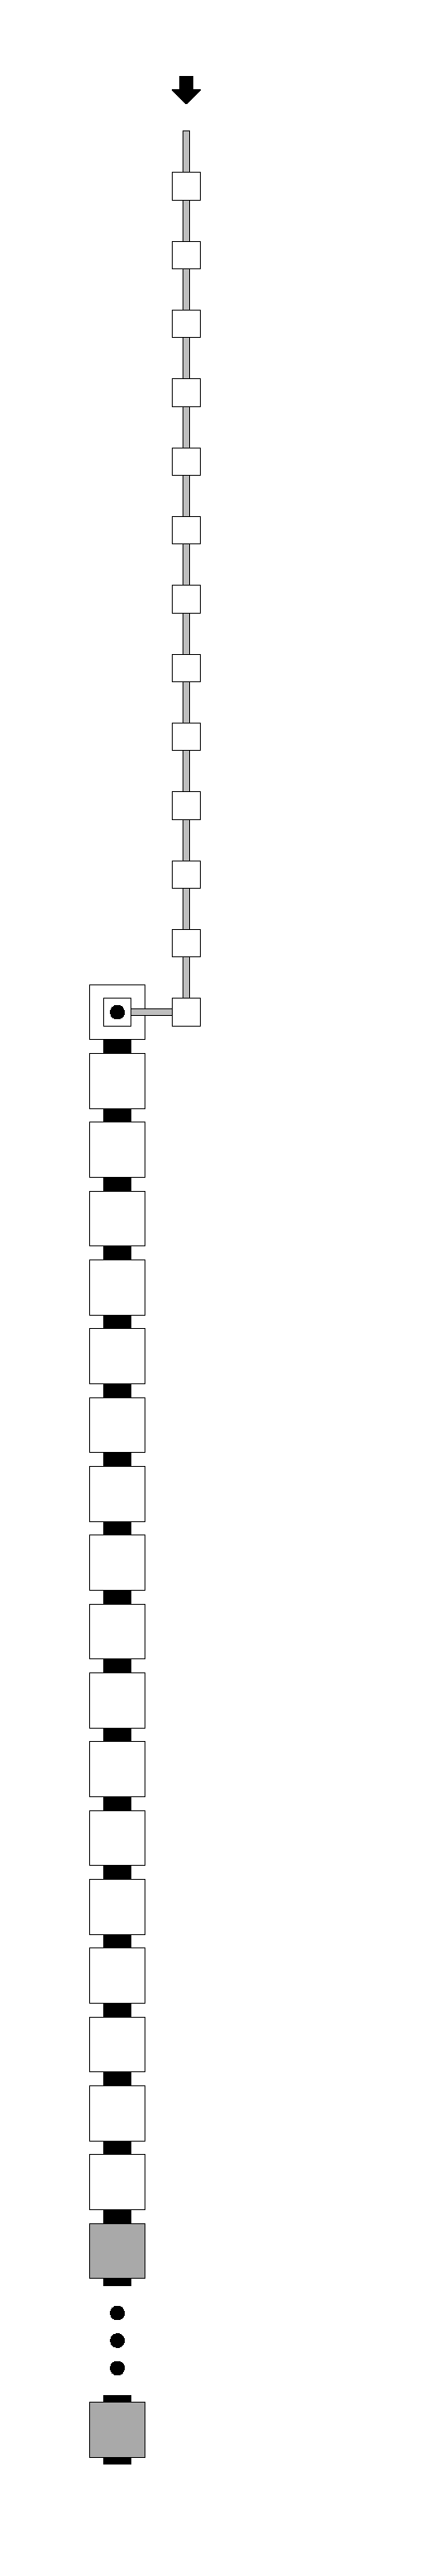
\includegraphics[width=0.32\textwidth]{return_paths_return_from_digit_2_op-or-seed}
        \caption{\label{fig:return_from_digit2_oporseed} General and initial value digit 2}
    \end{subfigure}%
    ~
    \begin{subfigure}[t]{0.32\textwidth}
        \centering
        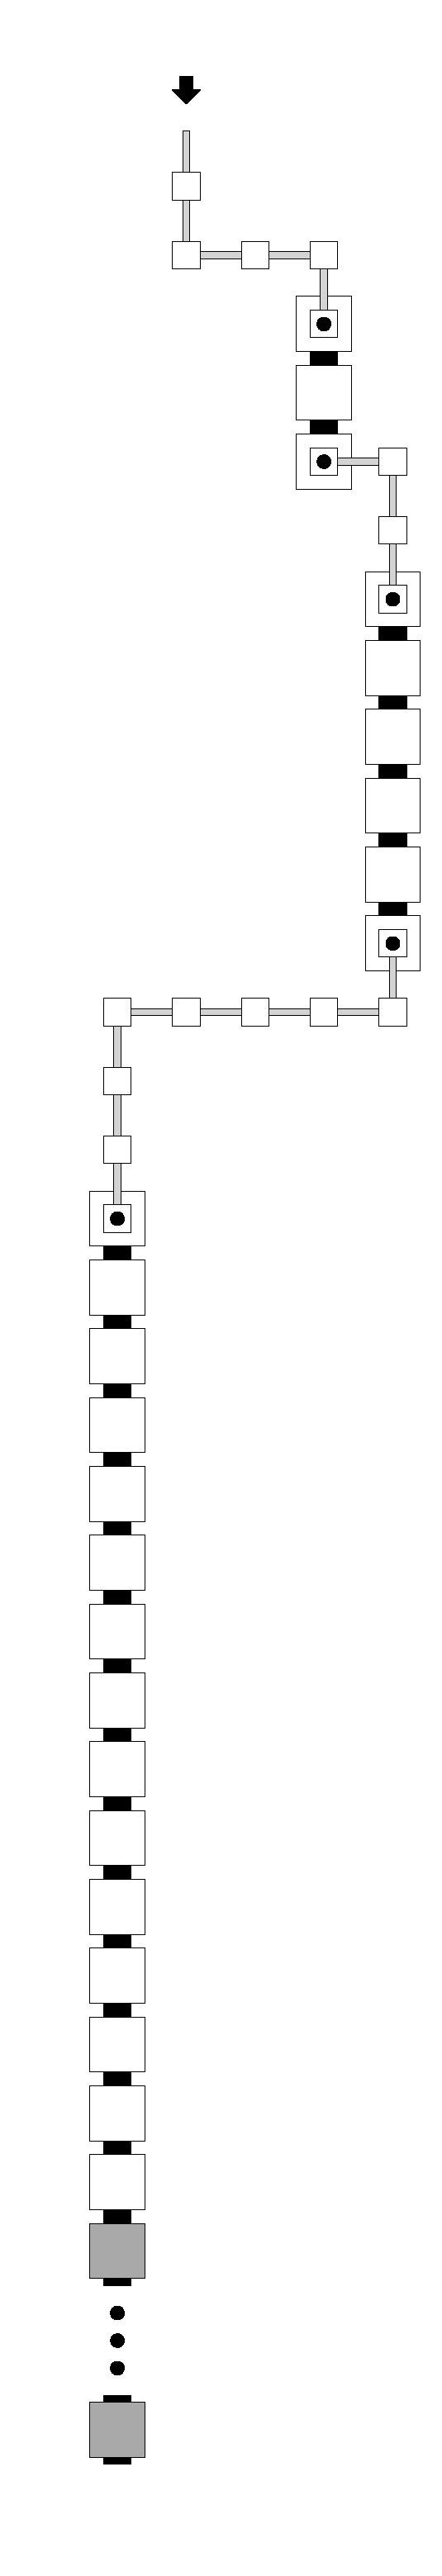
\includegraphics[width=0.32\textwidth]{return_paths_return_from_digit_1_op}
        \caption{\label{fig:return_from_digit_1_op} General digit 1}
    \end{subfigure}%
    ~
\end{figure}

\begin{figure}[H]\ContinuedFloat
    \centering
    \begin{subfigure}[t]{0.32\textwidth}
        \centering
        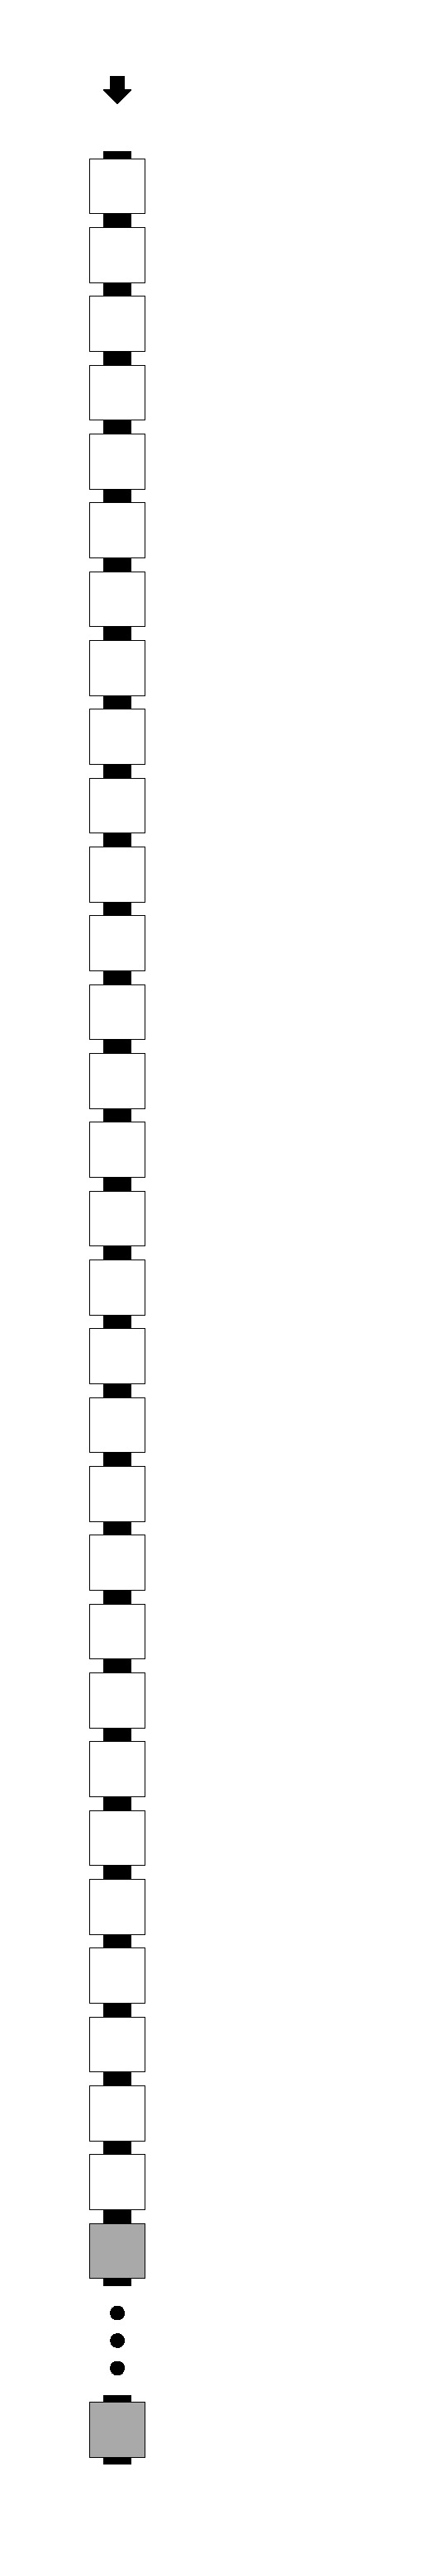
\includegraphics[width=0.32\textwidth]{return_paths_return_from_digit_1_op_msr}
        \caption{\label{fig:return_from_digit_1_op_msr} Digit 1 - case 2}
    \end{subfigure}%
    ~
    \begin{subfigure}[t]{0.32\textwidth}
        \centering
        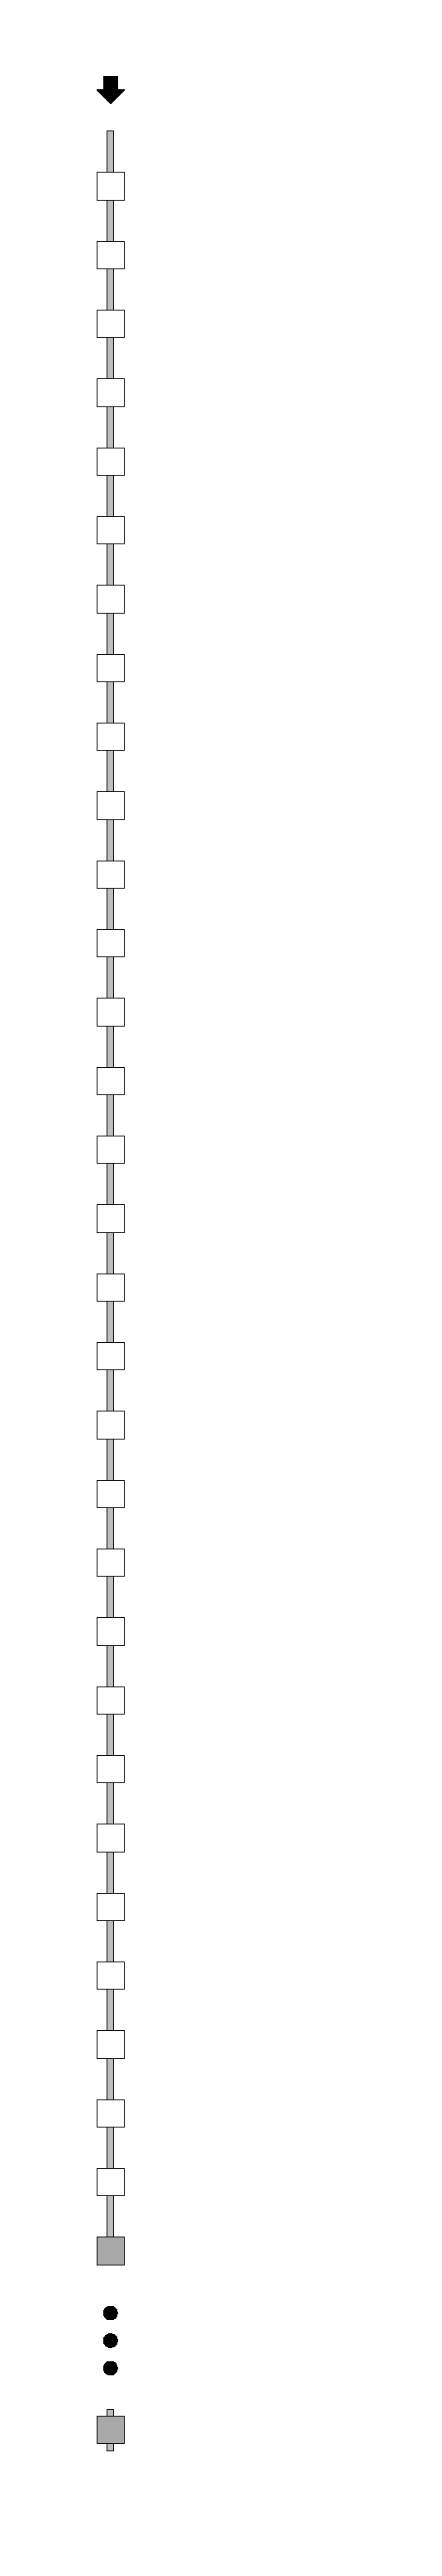
\includegraphics[width=0.32\textwidth]{return_paths_return_from_digit_1-or-2_op_msr_msd}
        \caption{\label{fig:return_from_digit_1or2_op_msr_msd} MSD - Digit 1 and 2 }
    \end{subfigure}%
    \caption{\label{fig:return_from_digits} The {\returnfromdigit} gadgets for digits 1 and 2}
\end{figure}

\begin{figure}[H]
    \centering
    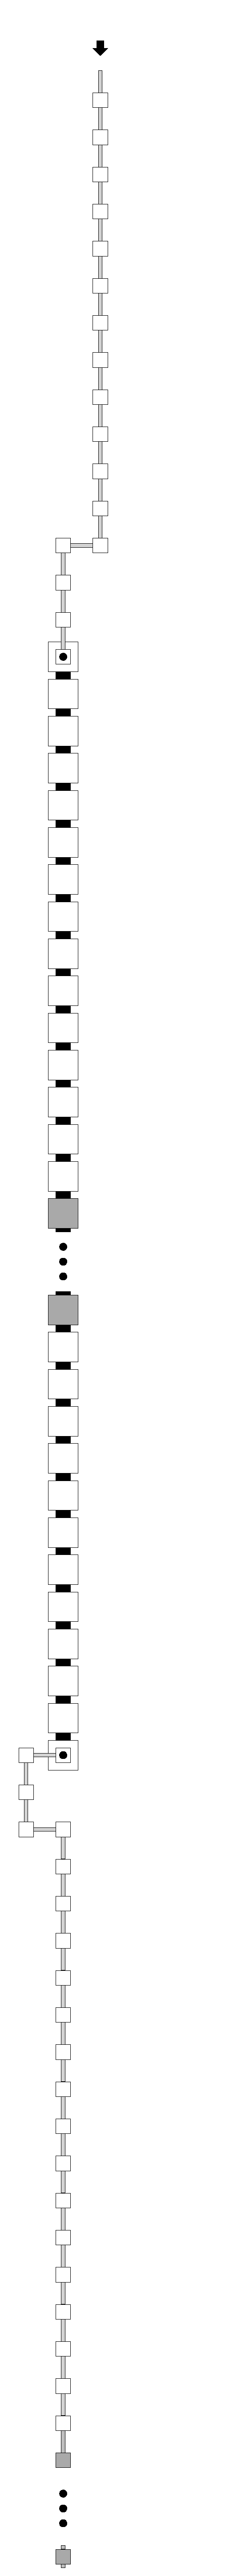
\includegraphics[width=0.08\textwidth]{return_paths_return_from_digit_3}
    \caption{\label{fig:return_from_digit_3} The {\returnfromdigit} gadget for digit 3.}
\end{figure}


The first part of the return paths is the {\returnfromdigit} micro-gadget.

For each $\inc\in \{ {\tt increment}, {\tt copy} \}$:

\begin{itemize}

    % DIGIT 1
    \item Create
    $\begin{aligned}[t]
        \returnfromdigit(& \left\langle \returnpath,    1, \inc \right\rangle,
                           \left\langle {\tt NextRead}, 1, \inc \right\rangle \;)
    \end{aligned}$\\from the micro-gadget shown in Figure~\ref{fig:return_from_digit_1_op}.

    \item Create
    $\begin{aligned}[t]
        \returnfromdigit(& \left\langle \returnpath,    1, \inc, {\tt msr} \right\rangle,
                           \left\langle {\tt NextRead}, 1, \inc, {\tt msr} \right\rangle \;)
    \end{aligned}$\\from the micro-gadget shown in Figure~\ref{fig:return_from_digit_1_op_msr}

    \item Create
    $\begin{aligned}[t]
        \returnfromdigit(& \left\langle \returnpath,    1, \inc, {\tt msr}, {\tt msd} \right\rangle,
                           \left\langle {\tt NextRead}, 1, \inc, {\tt msr}, {\tt msd} \right\rangle \;)
    \end{aligned}$\\from the micro-gadget shown in Figure~\ref{fig:return_from_digit_1or2_op_msr_msd}.



    % DIGIT 2
    \item Create
    $\begin{aligned}[t]
        \returnfromdigit(& \left\langle \returnpath,    2, \inc \right\rangle,
                           \left\langle {\tt NextRead}, 2, \inc \right\rangle \;)
    \end{aligned}$\\from the micro-gadget shown in Figure~\ref{fig:return_from_digit2_oporseed}.

    \item Create
    $\begin{aligned}[t]
        \returnfromdigit(& \left\langle \returnpath,    2, \inc, {\tt msr}, {\tt msd} \right\rangle,
                           \left\langle {\tt NextRead}, 2, \inc, {\tt msr}, {\tt msd} \right\rangle \;)
    \end{aligned}$\\from the micro-gadget shown in Figure~\ref{fig:return_from_digit_1or2_op_msr_msd}.



    % DIGIT 3
    \item Create
    $\begin{aligned}[t]
        \returnfromdigit(& \left\langle \returnpath,    3, \inc \right\rangle,
                           \left\langle {\tt NextRead}, 3, \inc \right\rangle \;)
    \end{aligned}$\\from the micro-gadget shown in Figure~\ref{fig:return_from_digit_3}.

    \item Create
    $\begin{aligned}[t]
        \returnfromdigit(& \left\langle \returnpath,    3, \inc, {\tt msr}, {\tt msd} \right\rangle,
                           \left\langle {\tt NextRead}, 3, \inc, {\tt msr}, {\tt msd} \right\rangle \;)
    \end{aligned}$\\from the micro-gadget shown in Figure~\ref{fig:return_from_digit_3}.

\end{itemize}


The second part of the return gadgets is the {\readnext} micro-gadget. These gadgets output a blank {\cwrite}
signal if the counter should read the preceding digit in the current row.


\begin{figure}[H]
    \centering
    \begin{minipage}[b]{.64\textwidth}
        \centering
        \begin{subfigure}[t]{0.3\textwidth}
            \centering
            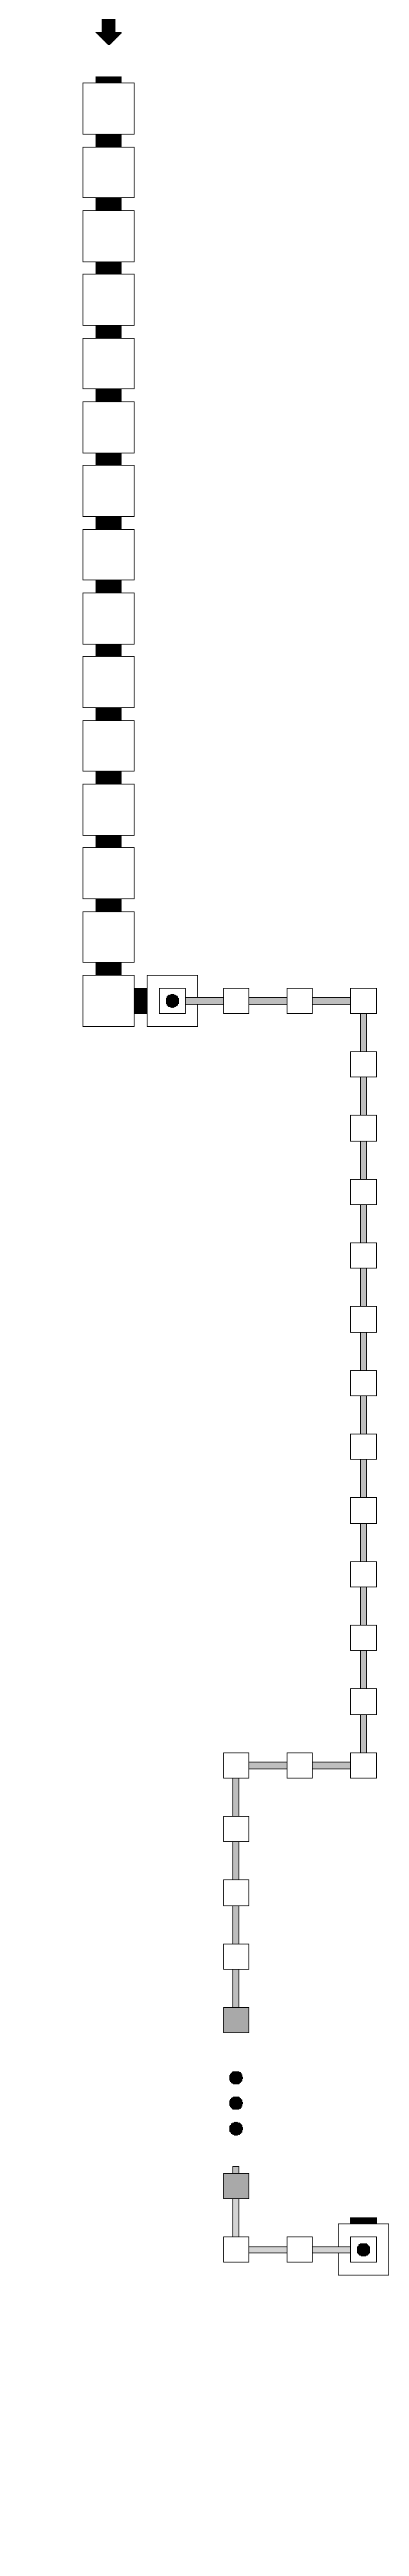
\includegraphics[width=.3\textwidth]{return_paths_read_next_1-or-2_op}
            \caption{\label{fig:read_next_1or2_op}}
        \end{subfigure}%
        ~
        \begin{subfigure}[t]{0.3\textwidth}
            \centering
            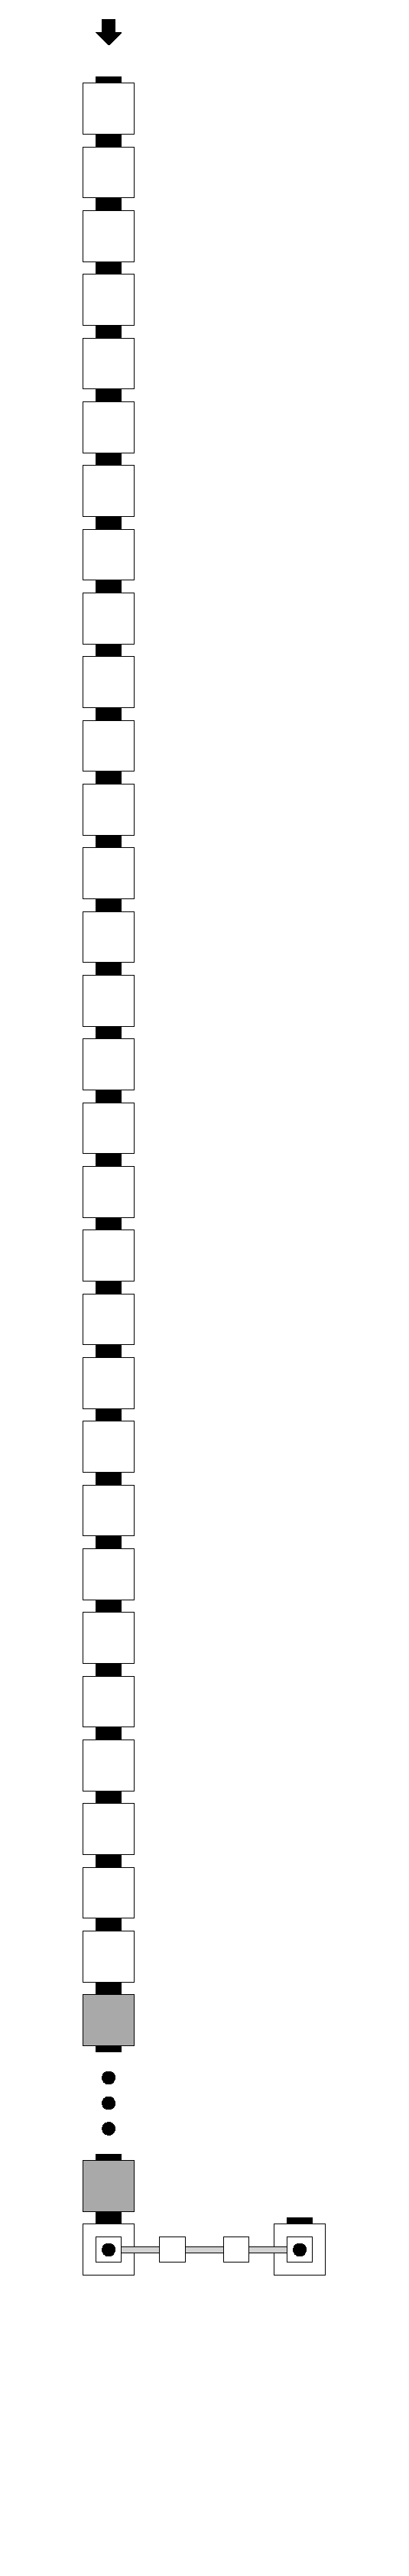
\includegraphics[width=0.3\textwidth]{return_paths_read_next_1_op_msr}
            \caption{\label{fig:read_next_1_op_msr}}
        \end{subfigure}%
        ~

        \begin{subfigure}[t]{0.3\textwidth}
            \centering
            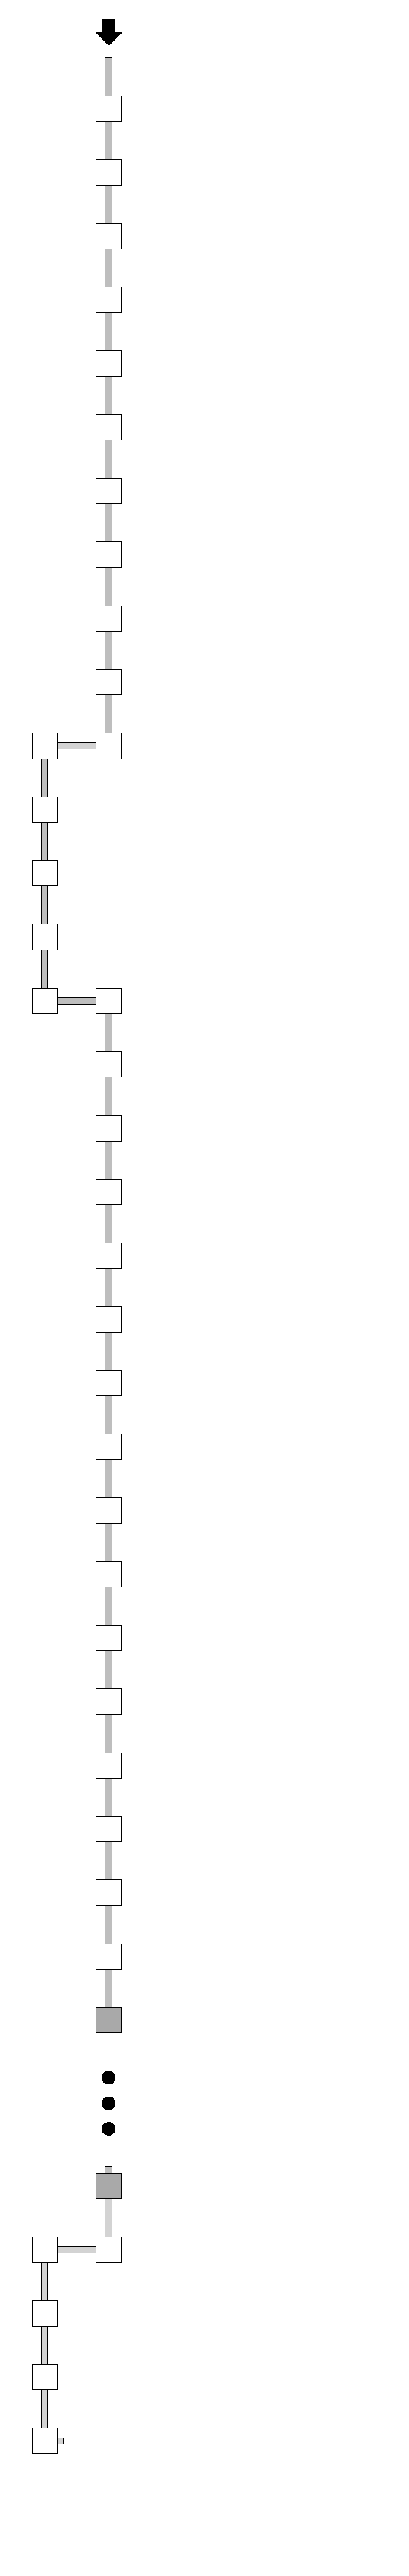
\includegraphics[width=0.3\textwidth]{return_paths_read_next_1-or-2_op_msr_msd}
            \caption{\label{fig:read_next_1or2_op_msr_msd}}
        \end{subfigure}%
        ~
        \begin{subfigure}[t]{0.3\textwidth}
            \centering
            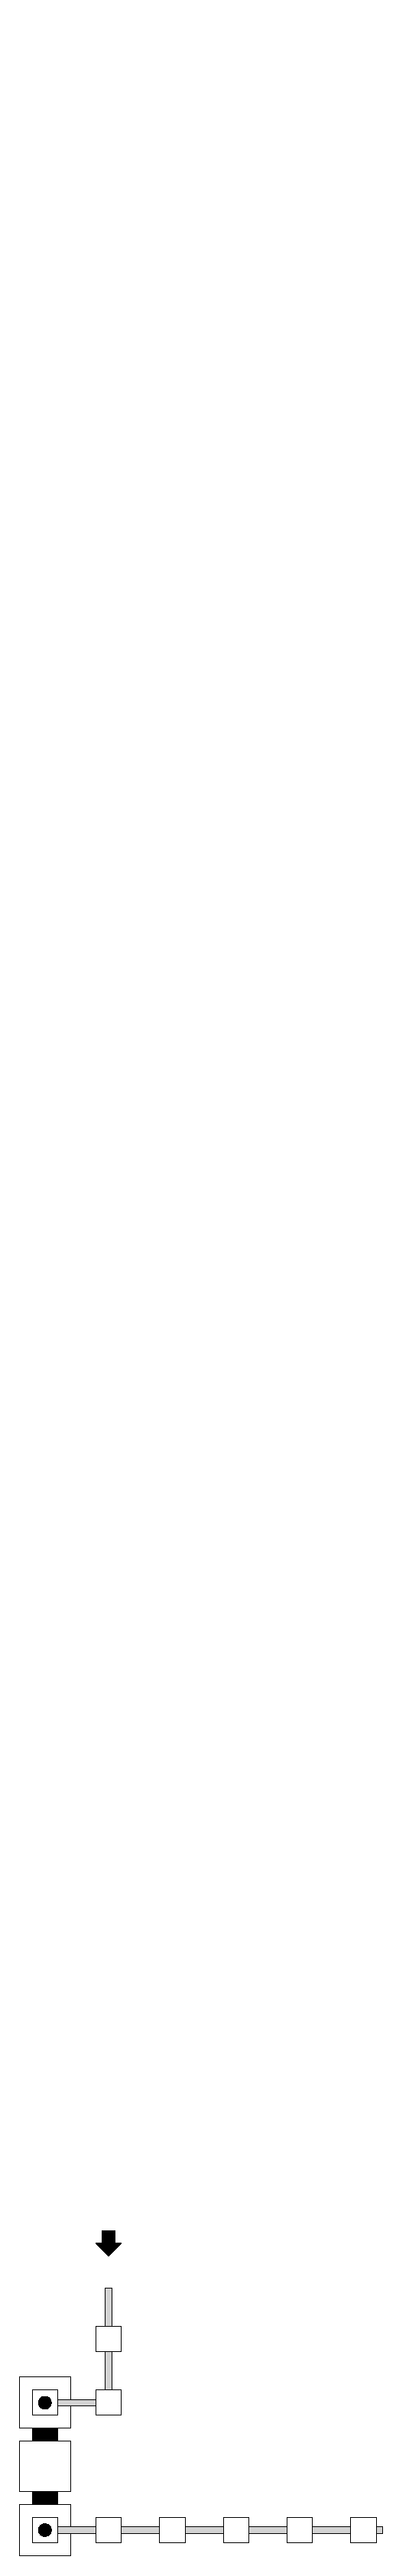
\includegraphics[width=0.3\textwidth]{return_paths_read_next_3_op-or-seed_msr_msd}
            \caption{\label{fig:read_next_3_oporseed_msr_msd}}
        \end{subfigure}%
        ~

        \begin{subfigure}[t]{0.3\textwidth}
            \centering
            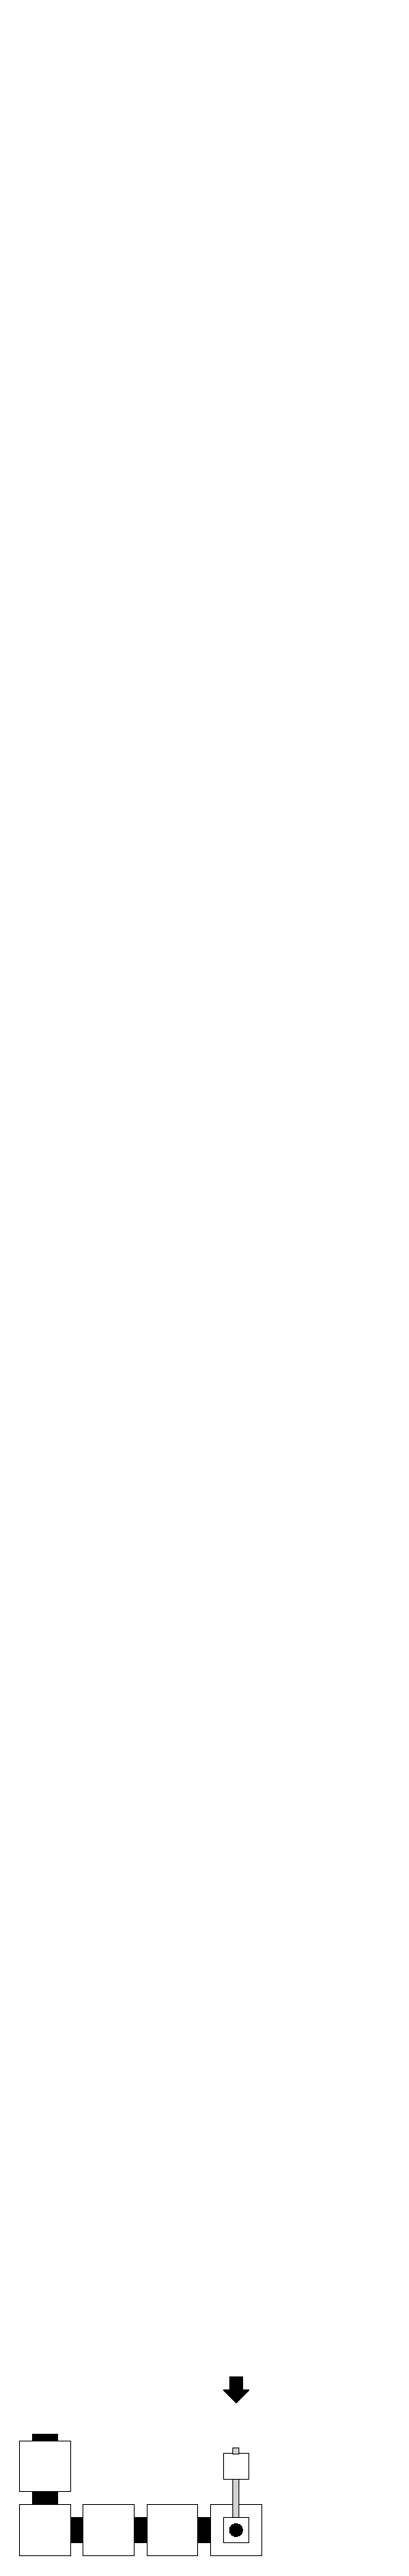
\includegraphics[width=0.3\textwidth]{return_paths_read_next_3_seed}
            \caption{\label{fig:read_next_3_seed}}
        \end{subfigure}%
        ~
        \begin{subfigure}[t]{0.3\textwidth}
            \centering
            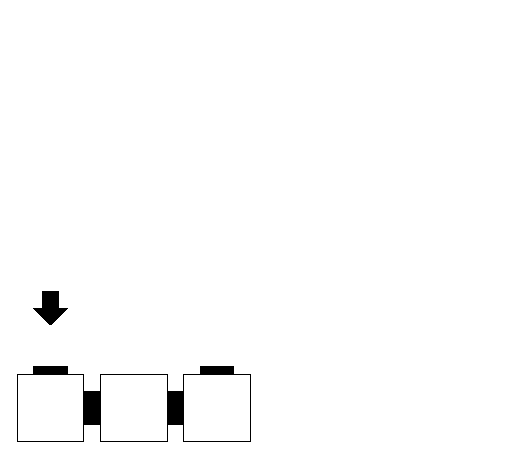
\includegraphics[width=0.3\textwidth]{return_paths_read_next_2_seed}
            \caption{\label{fig:read_next_2_seed}}
        \end{subfigure}%
        ~
    \end{minipage}%
    \begin{minipage}[b]{.35\textwidth}
      \centering
      \begin{subfigure}[t]{\textwidth}
        \centering
        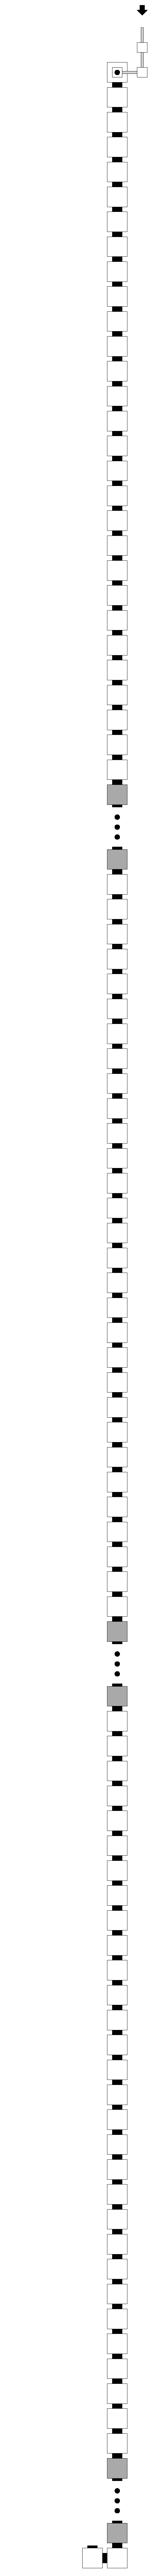
\includegraphics[width=.205\textwidth]{return_paths_read_next_3_op}
        \caption{\label{fig:read_next_3_op}}
      \end{subfigure}%
    \end{minipage}
    \caption{\label{fig:readnext} The {\readnext} gadgets}
\end{figure}

For each $\inc\in \{ {\tt increment}, {\tt copy} \}$:
\begin{itemize}

    % DIGIT 1
    \item Create
    $\begin{aligned}[t]
        \readnext(& \left\langle {\tt NextRead}, 1,          \inc \right\rangle,
                    \left\langle {\tt Read},     2, \lambda, \inc \right\rangle \;)
    \end{aligned}$\\from the micro-gadget shown in Figure~\ref{fig:read_next_1or2_op}.

    \item Create
    $\begin{aligned}[t]
        \readnext(& \left\langle {\tt NextRead}, 1,          \inc, {\tt msr} \right\rangle,
                    \left\langle {\tt Read},     2, \lambda, \inc            \right\rangle \;)
    \end{aligned}$\\from the micro-gadget shown in Figure~\ref{fig:read_next_1_op_msr}.

    \item Create
    $\begin{aligned}[t]
        \readnext(& \left\langle {\tt NextRead}, 1,      \inc, {\tt msr}, {\tt msd} \right\rangle,
                    \left\langle {\tt Cross\_Next\_Row}, \inc                       \right\rangle \;)
    \end{aligned}$\\from the micro-gadget shown in Figure~\ref{fig:read_next_1or2_op_msr_msd}.


    % DIGIT 2


    \item Create
    $\begin{aligned}[t]
        \readnext(& \left\langle {\tt NextRead}, 2,          \inc \right\rangle,
                    \left\langle {\tt Read},     3, \lambda, \inc \right\rangle \;)
    \end{aligned}$\\from the micro-gadget shown in Figure~\ref{fig:read_next_1or2_op}.

    \item Create
    $\begin{aligned}[t]
        \readnext(& \left\langle {\tt NextRead}, 2,      \inc, {\tt msr}, {\tt msd} \right\rangle,
                    \left\langle {\tt Cross\_Next\_Row}, \inc                       \right\rangle \;)
    \end{aligned}$\\from the micro-gadget shown in Figure~\ref{fig:read_next_1or2_op_msr_msd}.


    % DIGIT 3
    \item Create
    $\begin{aligned}[t]
        \readnext(& \left\langle {\tt NextRead}, 3,          \inc \right\rangle,
                    \left\langle {\tt Read},     1, \lambda, \inc \right\rangle \;)
    \end{aligned}$\\from the micro-gadget shown in Figure~\ref{fig:read_next_3_op}.

    \item Create
    $\begin{aligned}[t]
        \readnext(& \left\langle {\tt NextRead}, 3,      \inc, {\tt msr}, {\tt msd} \right\rangle,
                    \left\langle {\tt Cross\_Next\_Row}, \inc \right\rangle \;)
    \end{aligned}$\\from the micro-gadget shown in Figure~\ref{fig:read_next_3_oporseed_msr_msd}.


\end{itemize}

\subsubsection{Cross over gadget}

The idea this gadget is to assemble after reading the MSD, and route the
counter to back to the start of the next row, in position for the counter to
begin reading the first digit. The number of tiles shaded in darker grey is
$6 \cdot \floor*{\frac{d}{3}}$.

\vspace{.5cm}
For each $\inc\in \{ {\tt increment}, {\tt copy} \}$:

\begin{itemize}
    \item Create
    $\begin{aligned}[t]
        {\tt Crosser}(&\left\langle {\tt Cross\_Next\_Row}, \inc \right\rangle,
                       \left\langle {\tt Read}, 1, \lambda, \inc \right\rangle \;)
    \end{aligned}$\\from the micro-gadget shown in Figure~\ref{fig:cross_to_next_row}.
\end{itemize}


\begin{figure}[H]
    \centering
    \subcaptionbox{General \label{fig:cross_to_next_row}}
    {\makebox[0.24\textwidth][c]{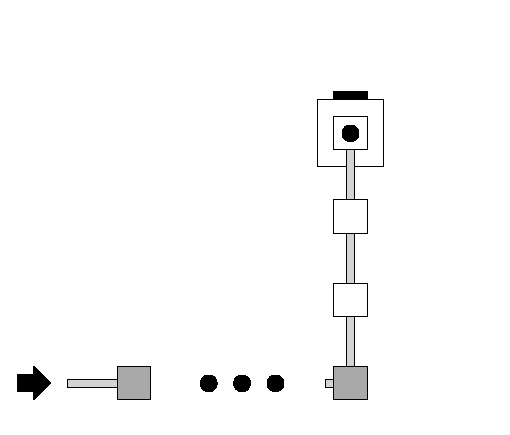
\includegraphics[width=1in]{cross_to_next_row}}}%
    ~
    \subcaptionbox{General overview \label{fig:cross_next_row_overview}}
    {\makebox[0.24\textwidth][c]{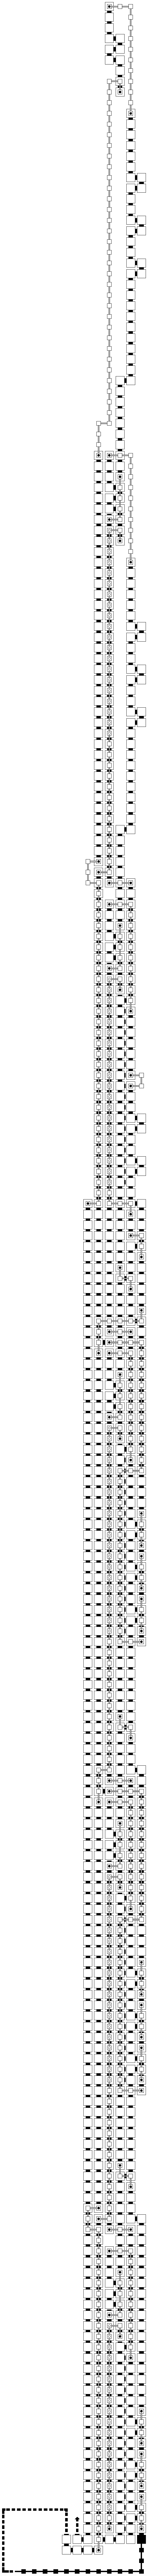
\includegraphics[width=0.45in]{overviews/general/crosser}}}%
    ~
    \caption{\label{fig:crosser_gadgets} The {\tt Cross\_Next\_Row} gadget.}
\end{figure}